%!TEX root = ../seminararbeit.tex
\newpage
\section{Theorie: Kriterien zur Ideenbewertung}\label{sec:theorie}
Ideen zu bewerten ist ein wichtiger Schritt in der Entwicklung neuer Produkte. 
Auch in der Weiterentwicklung bereits existierender Lösungen darf eine Bewertung im Entwicklungsprozess nicht fehlen. 
Durch Ideenfindungsmethoden, wie zum Beispiel Brainstorming, werden sehr viele Ideen generiert. Doch diese Ideen 
sind oft nicht alle zielführend. 
Durch Bewertung und Kategorisierung können die vielversprechendsten Ideen aus einer großen Menge heraus gefiltert werden. 
Sich auf zielführende Ideen zu fokussieren, hat besonders wirtschaftliche Gründe.
Je mehr Zeit vergeht, bis eine Idee als nicht umsetzbar oder nicht zielführend erkannt wird, desto mehr Kosten muss das Unternehmen tragen.
Ziel der Ideenbewertung ist es, Ideen frühzeitig zu filtern, um so das Risiko misslungener Investitionen zu vermeiden.
\cite{grossklaus:2008}\\
\autoref{img:filterKosten} zeigt eine Statistik, die die steigenden Kosten bei fortschreiten der Entwicklung zeigt. 
\begin{figure}[h]
	\centering
	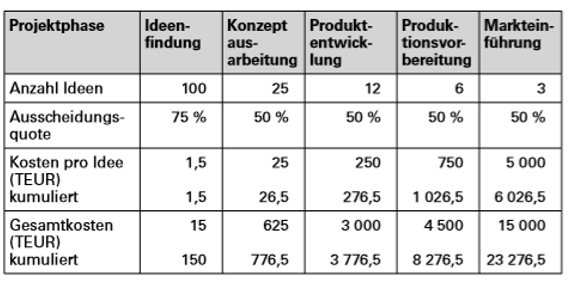
\includegraphics[width=10cm]{ideenfilterung.png}
	\caption{Ausscheidungsquoten und Kostenentwicklung}
	\label{img:filterKosten}
\end{figure}

\subsection{Ideenbewertung}
Der Kern einer Ideenbewertung sind die Kriterien, anhand derer über eine Idee geurteilt wird.
Aus diesem Grund ist es wichtig, die Kriterien sorgfältig zu definieren. Werden die Kriterien falsch oder nicht sorgfältig gewählt,
so kann dies zu Ablehnungs- oder Annahmefehlern führen. 
Ablehnungsfehler bezeichnen Ideen, die fälschlicherweise abgelehnt wurden, obwohl sie bei genauerer Betrachtung 
zielführend gewesen wären. Das Gegenteil sind Annahmefehler, hier wird eine Idee weiterverfolgt, obwohl diese nicht zum Ziel führt. 
Während Ablehnungsfehler zu einer Verzögerung in der Entwicklung führen können, hinterlassen Annahmefehler verschwendete Zeit und verschwendetes Geld.\\

Kriterien lassen sich grundsätzlich in zwei Kategorien unterteilen. Allgemeine Kriterien und aufgabenspezifische Kriterien.\\
\textbf{Allgemeine Kriterien} lassen sich auf verschiedene Ideen und Anwendungsfälle übertragen.
Um allgemeine Kriterien zu definieren, ist es nicht notwendig, die konkrete Aufgabe zu kennen. 
Die häufigsten allgemeinen Kriterien sind \textit{Attraktivität}, \textit{Realisierbarkeit} und 
\textit{Disruptionspotential}. Es ist erkennbar, dass es sich hierbei um grundsätzliche Kriterien handelt, die unabhängig von einer Thematik sind.\\
\textbf{Aufgabenspezifische Kriterien} hingegen erfordern genaue Kenntnisse der Aufgabenstellung. Es muss klar sein, welches 
konkrete Kundenbedürfnis mit einer Idee befriedigt werden soll. Auch verschiedene Markttrends müssen hierbei beachtet werden. 
Diese haben oft entscheidenden Einfluss auf die Erfolgschancen. Aufgabenspezifische Kriterien müssen für jede Aufgabe und jedes Ziel 
individuell formuliert werden.
\cite{grossklaus:2008}

\subsection{Kriterien der Ideenbewertung nach Zephram}
Auch Zephram teilt die Kriterien in zwei Kategorien ein. Allerdings setzt Zephram einen anderen Fokus und verfolgt 
damit ein anderes Ziel.\\

\textbf{Randbedingungen} beschreiben die Eigenschaften, die eine Idee haben muss
beziehungsweise nicht haben darf. Sie sind absolut und werden oft als \textit{Muss-Kriterien}
und \textit{Darf-Nicht-Kriterien} bezeichnet.
Typische Randbedingungen sind beispielsweise die \textit{Kosten}. 
Es wird festgelegt welchen Betrag eine Ideenumsetzung maximal kosten darf. 
Weitere typische Randbedingungen sind \textit{Fit}, die Idee muss zum Unternehmensimage passen, oder \textit{Ressourcen}, die Ressourcen für die
Umsetzung müssen vorhanden sein. 
Randbedingungen sind entweder erfüllt oder nicht erfüllt. Je nachdem wird eine Idee verworfen oder weiterverfolgt. \\

\textbf{Erfolgskriterien} hingegen sind nicht absolut. Sie beschreiben Eigenschaften einer Idee, 
mit denen diese als erfolgreich gilt. Ziel ist es nicht, Ideen auszuschließen, sondern die
vielversprechendste Idee herauszufiltern. Das heißt im Umkehrschluss, alle anderen Ideen werden nicht 
verworfen, sondern zunächst nicht ausgewählt. Erfolgskriterien werden oft als \textit{Soll-Kriterien} bezeichnet. Um 
Erfolgskriterien einheitlich zu formulieren kann der Satz \textit{"Je mehr..., desto besser"} verwendet werden.
Dieser Satz verdeutlicht, dass sich Erfolgskriterien nicht in \textit{erfüllt} und \textit{nicht erfüllt} aufteilen 
lassen. Typische Erfolgskriterien sind \textit{Gewinnpotential}, \textit{Wachstumspotential} oder \textit{Kundennutzen}.\\

\textbf{Kann-Kriterien} sollten bei der Bewertung von Ideen keine Rolle spielen. Es handelt sich hierbei 
um Kriterien, die nicht zwingend notwendig für den Erfolg einer Idee sind. Wird eine Idee anhand dieser Kriterien 
bewertet, so sind die Erfolgskriterien nicht gut gewählt und sollten demnach angepasst werden.\\

Beim \textbf{Formulieren} der Randbedingungen ist es wichtig, dass sich die Kriterien nicht
widersprechen. Die Folge wäre, dass alle Ideen aussortiert werden, da niemals alle Randbedingungen erfüllt sein können.
Als häufiges Beispiel ist hier die Forderung nach einer Systemausfallsicherheit von 98\% , bei einer
kurzer Entwicklungszeit. 
Es kommt bei den Kriterien darauf an, das richtige Mittelmaß für die Aufgabe zu finden. 
Sowohl Randbedingungen wie auch Erfolgskriterien sollten zur Aufgabe passen. Beide Kriterienarten sind im 
Bereich der aufgabenspezifischen Kriterien. Eine weitere Schwierigkeit ist eine möglichst konkrete
Formulierung der Kriterien zu finden. \\

Beim \textbf{Anwenden} der Kriterien zur Bewertung von Ideen müssen zunächst die Randbedingungen angewandt werden. 
Dies sorgt bereits für eine starke Reduktion der Ideenanzahl. Um hierbei keine Fehler zu machen, wird 
ein Vier-Augen-Prinzip empfohlen. 
Schwieriger ist die anschließende Anwendung der Erfolgskriterien, da diese graduell sind, allerdings keine klar 
definierte Messskala besitzen. 
Es gibt einige Methoden, die die Arbeit mit Erfolgskriterien vereinfachen. Einige werden 
in der folgenden Liste aufgezählt: 
\begin{itemize}
    \item Punktekleben (Siehe in Kapitel \ref{sec:retro-punkte})
    \item Nutzwertanalyse
    \item Paarvergleichsmatrix
\end{itemize}
Die Methoden die von \ac{sac} angewendet werden, werden im Praxisteil genauer beschrieben. \cite{zephram:2018}

\subsection{Vorgehensweise nach Schawel-Billing}
Vorschlag von Schawel und Billing ist es, die Ideenbewertung in zwei Phasen zu unterteilen. Zunächst muss die gesamte Anzahl 
der Ideen verringert werden. Dies geschieht in der \textbf{Ideenkategorisierung}. Hierbei geht es darum, Ideen unter 
Oberbegriffen zusammenzufassen. Dies hilft vorallem dabei, ähnliche Ideen oder Überlappungen frühzeitig zu erkennen.
Zusätzlich hat diese Vorgehensweise den Vorteil, dass die gefundenen Kategorien später in Arbeitspakete überführt werden 
könnten. Anschließend können die Kategorien in der \textbf{Ideenbewertung} genauer Bewertet werden. 
Dies erfolgt anhand formulierter Kriterien. Für eine erste Einschätzung kann außerdem eine \ac{2d}-Matrix verwendet werden. 
Diese sollte die beiden Achsen \textit{Wirkung} und \textit{Realisierbarkeit} entgegenstellen. Ideen die eine geringe Wirkung haben und/oder 
schwer zu realisieren sind können so leicht identifiziert werden. \cite{schawel:2009}